\section{Optimization with Gradient Descent}\label{gd}
All throughout Machine Learning gradient descent and variations of it are used for optimization. Gradient descent is vital for my work. As such I will briefly explain what it is and how it is relevant to my work.

\subsection{What is Gradient Descent?}\label{gd:what_is_it}
In essence gradient descent is an algorithm used to find local minima of differentiable functions. It can be thought of as starting at a point on the function graph and walking down hill until one reaches a minimum. Gradient descent works by differentiating a function at some point in order to obtain a slope, and then moving in the downwards direction of that slope. Gradient descent is done in steps. If $f(\theta)$ is a differentiable function, then one gradient descent step is:

\begin{equation}\label{Graident_Descent:basic_update}
    \theta \leftarrow \theta - \alpha \cdot \frac{\partial}{\partial \theta}f(\theta)
\end{equation}

\noindent
\\ The \textit{step size} $\alpha$ is introduced to control the magnitude of the descent step. The gradient descent algorithm consists of performing these steps iteratively until the current value (in the above case $\theta$) is sufficiently close to the actual local minimum. Performing 10 gradient descent steps on the function $f(\theta) = \theta^2$ and a starting value of $\theta = 3$ with various values for alpha looks as follows:

\begin{figure}[ht]
    \centering
    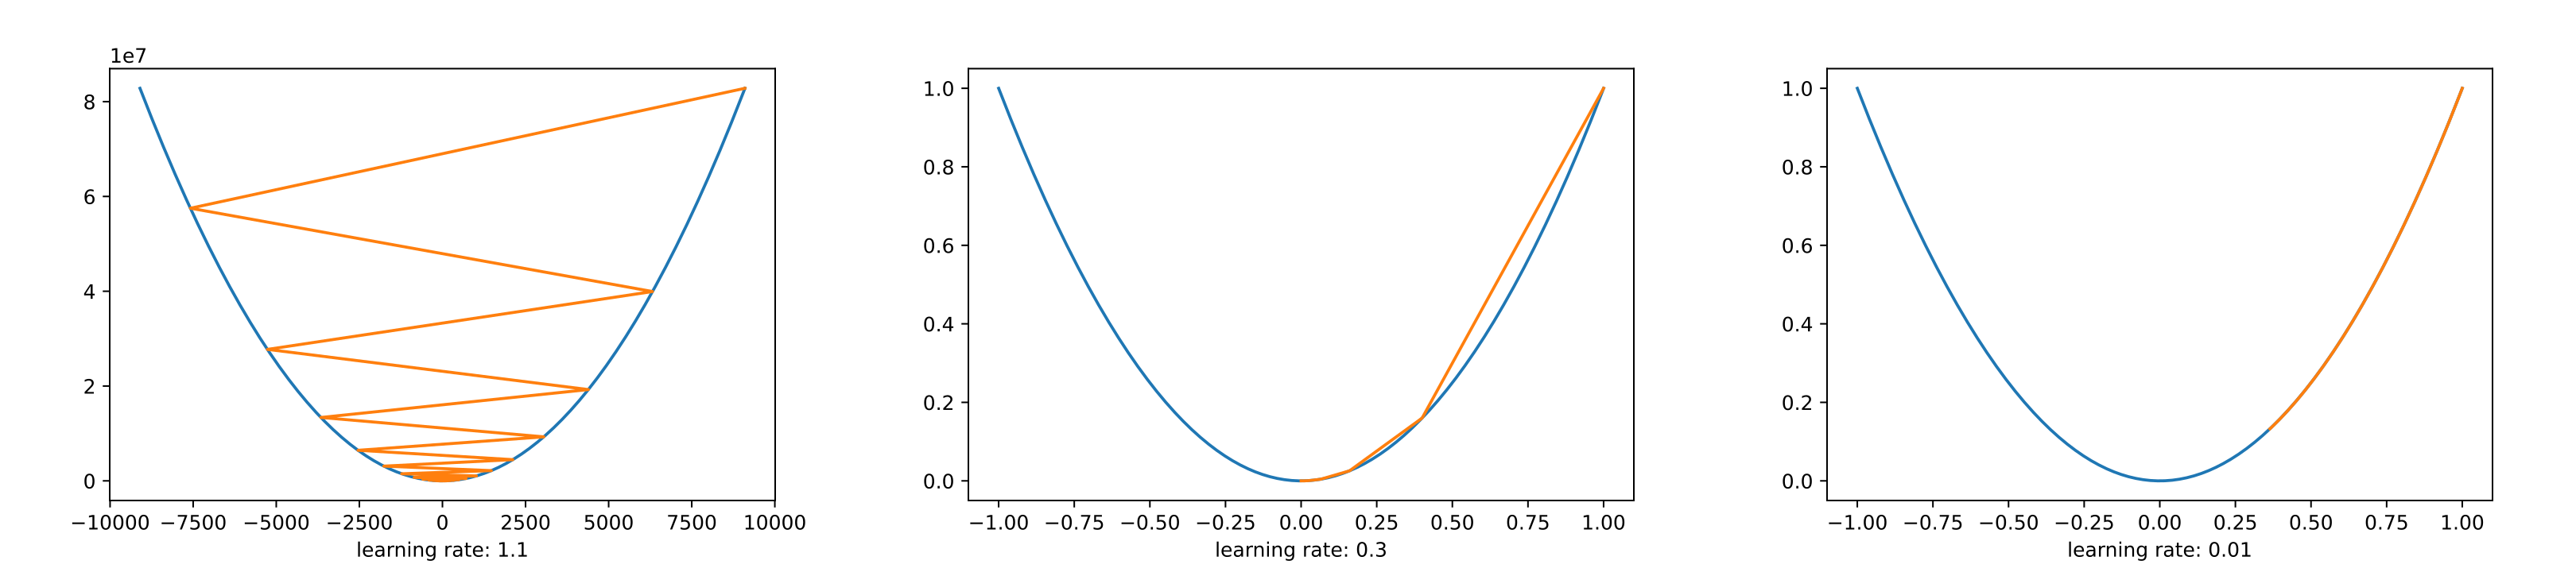
\includegraphics[width=\linewidth]{figures/grad_desc.png}
    \caption{Gradient Descent on $f(\theta) = \theta^2$}
    \label{fig:UNO}
\end{figure}

\noindent
\\ As can be clearly seen here smaller step sizes lead to more accurate results. Too large a step size may even lead to divergence. However, if the step size is too small, it may take very long to reach a local minimum. Gradient descent functions in the exact same way if $\theta$ is a vector. In that case the update step becomes:

\begin{equation}\label{Graident_Descent:basic_update_vector}
    \theta \leftarrow \theta - \alpha \cdot \nabla_\theta f(\theta)
\end{equation}

\subsubsection{Gradient Ascent}\label{gd:gradient_ascent}
As the name implies gradient ascent is the exact opposite of gradient descent. Instead of trying to find the local minimum of a function, when performing gradient ascent we are trying to find the local maximum of a function. Gradient Ascent is identical to performing Gradient Descent on the negative derivatives. 

\subsection{How is Gradient Descent relevant to Reinforcement Learning?}\label{gd:relevance}
In the previous section we have established that policies are functions which take actions and produce probability distributions over a set of actions. They may also be parameterized. One very common way of optimizing policies is to define a function $J(\theta)$, which measures agent performance \citepg{312}. This function is dependant on, and differentiable with respect to, the policy parameters $\theta$. Gradient Descent or Ascent (which one we use is dependant on if the performance measuring function treats lower or larger values as better) can then be used to optimize $\theta$. I will present one such function, in section \ref{sec:policy_gradient}. Gathering a set of agent-environment interactions, using the rewards received in them in a performance measuring function which depends on the policy parameters, and then using a variation on Gradient Descent to optimize those parameters, is the method i use to train an agent in this thesis. 

\subsection{Improvements on Gradient Descent}\label{subsec:gd:adam}
To achieve satisfactory performance the baseline gradient descent algorithm presented above did not suffice. Instead I opted for a, all throughout machine learning widely used optimization algorithm, called Adam \cite[pg 305]{Goodfellow-et-al-2016}. It combines a number of improvements on gradient descent, they are extensively covered in the pages preceding Adam in the book cited above. Basic gradient descent has a number of issues. The main way in which Adam improves on gradient descent, is by introducing momentum. In essence, a gradient using momentum can be thought of as the gradient averaged across a number of previous descent steps. This is useful since it allows for optimization past a local minimum, where regular gradient descent would get stuck. A common and useful analogy for this is a ball rolling down a hill. In regular gradient descent this ball would get stuck at even the smallest of local minima. However if that ball has momentum it might simply roll over such features of the parameter space. It also allows for carrying velocity through long flat sections where the gradients are relatively small, and would lead to unfeasibly long training times in Reinforcement Learning. The Adam optimization algorithm based on \cite[p. 306]{Goodfellow-et-al-2016}, and the original paper \cite{kingma2017adam} looks as follows:

\begin{algorithm}[H]
\DontPrintSemicolon
\SetAlgoLined
 \KwRequire{$\alpha$ Step size}
 \KwRequire{$\rho_1, \rho_2 \in \left[0, 1\right)$ Exponential decay rates for momentum estimates}
 \KwRequire{$\delta$ Small constant used for numerical stability}
 \KwRequire{$\theta_0$ Initial parameter vector}
 $m_0 \leftarrow 0$ (Initialize first moment vector)\;
 $v_0 \leftarrow 0$ (Initialize second moment vector)\;
 $t \leftarrow 0$ (Initialize timestep)\;
 \Repeat{$\theta_t$ converges}{
  $t \leftarrow t+1$\;
  $g_t \leftarrow \nabla_\theta f_t(\theta_{t-1})$ (Get gradients w.r.t. objective)\;
  $m_t \leftarrow \rho_1 * m_{t-1} + \left(1-\rho_1\right)\cdot g_t$ (Update first moment estimate)\;
  $v_t\leftarrow \rho_2 * m_{t-1} + \left(1-\rho_2\right)\cdot g_t \odot g_t$ (Update second moment estimate)\;
  $\hat{m}_t \leftarrow {m_t}/{\left(1-\rho_1^t\right)}$ (correct first moment for initial bias)\;
  $\hat{v}_t \leftarrow {v_t}/{\left(1-\rho_2^t\right)}$ (correct first moment for initial bias)\;
  $\theta_t \leftarrow \theta_{t-1} - \alpha \cdot {\hat{m}_t}/{\left(\sqrt{\hat{v}_t} + \delta \right)}$ (Update parameters)\;
 }
 \caption{The Adam algorithm}
\end{algorithm}
